\subsection{T3 Task 1. Code Representation Learning for DL-based Bug Detection (BD) Models}

We plan to use our Design Framework to advance CRL techniques
for DL-based BD approaches.
%a DL-based BD approach~\cite{yioopsla19}.
%We illustrate to improve current state-of-the-art BD approaches using
%effective code representation learning (CRL). Existing
%approaches~\cite{Pradel-2018,Wang-2016,Bian-2018,ayewah-2007} still
%have limitations in detecting bugs occurring multiple methods and
%suffer high false positive rates.
We designed a BD {\bf specialized CRL} {\em capturing contexts in
  method bodies and relations among methods}~\cite{yioopsla19}.  Our
initial design has three main steps (Figure~\ref{Fig.2}): (1)
\textbf{Attention-Based Local Context Representation Learning}.  
Our model extracts long paths over the AST built from the method's body.
%A path starts from a leaf node and ends at another leaf node and
%passes the root node of the AST, as the leaf nodes in an AST are
%terminal nodes with concrete lexemes.
The nodes in a path are encoded into a continuous vector via Word2Vec
and the vectors are fed into two layers: attention-based GRU (att-GRU)
layer~\cite{Cho-2014} and attention Convolutional (att-Conv)
layer~\cite{Yin-2016}. The GRU layer allows our model to encode and
emphasize on the order of the nodes in a path. The att-Conv layer
allows our model to emphasize and put more weights on buggy paths.
Then, we use Multi-Head Attention~\cite{Vaswani-2017} to combine the
result from att-GRU layer and att-Conv layer together as the
\textbf{path local context} representation.
%
\begin{wrapfigure}{r}{0.6\textwidth}
	\vspace{-13pt}
	\centering
	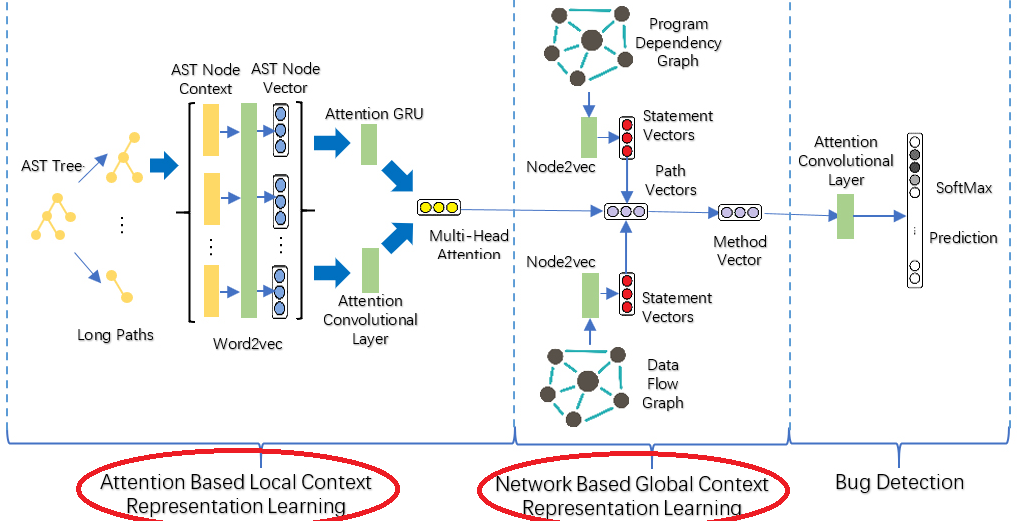
\includegraphics[height = 1.98in]{graphs/Graph_2_trim.png}
	\vspace{-22pt}
	\caption{Using Representation Learning for Bug Detection}
	\label{Fig.2}
%	\vspace{-10pt}
\end{wrapfigure}
(2) \textbf{Network-Based Global Context Representation Learning}.  We
also encode the method's context by building the PDG and the DFG
relevant to the method.
%We call them the \textbf{global context} as they provide the relations
%between the given method and other relevant methods in the project.
We use the Node2Vec~\cite{Grover-2016} to encode the PDG and DFG into
embedded vectors. These two vectors are combined by the space vectors
of all nodes in each path. We use matrix multiplication and convert
results together to get the path representation vector. Then, we can
have a method representation by appending all paths' vectors for each
method.  (3) \textbf{Bug Detection}. With both contexts for a method,
a classifier decides if the method is buggy or not. 

We plan to (1) investigate new CRL via our
framework to integrate program slices/reduction, symbolic traces, code
abstraction and intermediate representations; (2) explore new
embeddings and learning models for different level detection; (3) study new DL models on vectors from CRL to identify bugs.

%Our preliminary results~\cite{oopsla19} showed that with
%representation learning mechanisms (Figure~\ref{Fig.2}), our model
%significantly outperforms the one with the off-the-shelf
%Word2Vec-based CRL.

%\begin{wrapfigure}{r}{0.57\textwidth}
%	\vspace{-10pt}
%	\centering
%	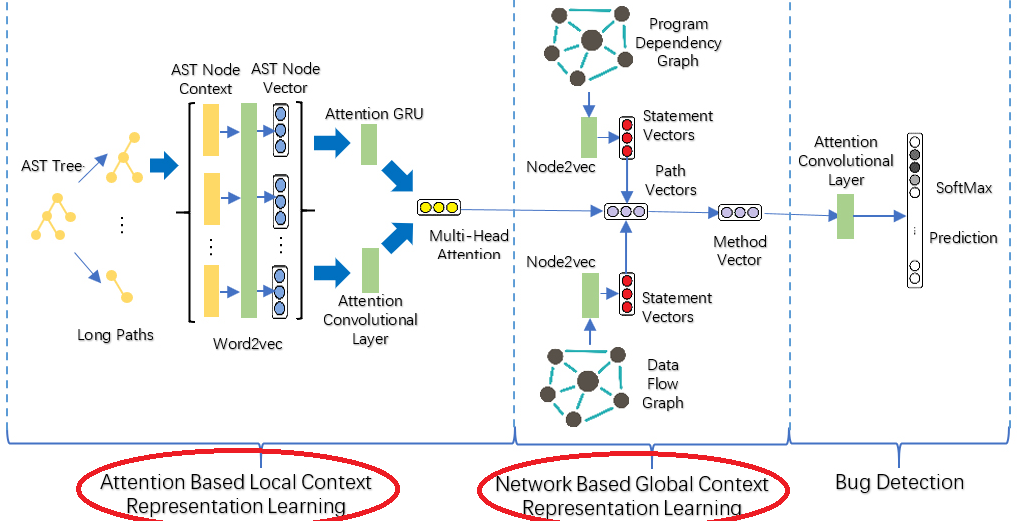
\includegraphics[scale=0.265]{graphs/Graph_2_trim.png}
%	\vspace{-25pt}
%	\caption{Using Representation Learning for Bug Detection}
%	\label{Fig.2}
%	\vspace{-15pt}
%\end{wrapfigure}

%Tien removed
%Table~\ref{allresults} show that (1) \textbf{our initial design
%  outperforms state-of-the-art baselines in detecting bugs},
%relatively improving DeepBugs, Bugram, NAR-miner, and FindBugs by
%69\%, 25\%, 92\%, and 156\% respectively in terms of F-score. (2)
%\textbf{our CRL with local and global contexts is more suitable than
%  existing CRL in bug detection}. It can improve relatively over all
%CLR baselines: DeepSim, DL-similarity, code2vec, Tree-based LSTM, Code
%Vectors,and GGM by 67\%, 38\%, 82\%, 206\%, 101\%, and 16.3\%,
%respectively, in terms of F-score. Importantly, our false positives
%rate is lower than others.
%\begin{wraptable}{r}{0.7\textwidth}
%	\vspace{-15pt}
%	{\footnotesize	
%		\caption{Ours Compared with BD Baselines and Existing CRL on BD. FP: False Positives}
%		\vspace{-10pt}
%		\begin{center}\label{allresults}
%			\renewcommand{\arraystretch}{1}
%			\begin{tabular}{p{1.2cm}<{\centering}|p{0.8cm}<{\centering}|p{0.8cm}<{\centering}|p{0.8cm}<{\centering}|p{1cm}<{\centering}|p{0.8cm}<{\centering}
%					|p{0.8cm}<{\centering}|p{0.8cm}<{\centering}|p{0.8cm}<{\centering}|p{0.8cm}<{\centering}|p{0.8cm}<{\centering}|p{0.8cm}<{\centering}} \cline{2-12}
%				
%				
%				\hline
%				\multirow{2}{*}{Category}& \multicolumn{5}{c|}{Bug detection baselines} & \multicolumn{6}{c}{Existing CRL on bug detection}\\
%				\cline{2-12}
%				& \textbf{Ours} & \textbf{DB} & \textbf{Bram} & \textbf{NARM} & \textbf{FB}   &\textbf{DS} & \textbf{DLS} & \textbf{C2V} & \textbf{TL} & \textbf{CV}&\textbf{GGM}\\
%				\hline
%				Recall  & 0.68 & 0.62 & 0.64 & 0.72 & 0.76   & 0.67 & 0.71 & 0.69 & \textbf{0.82} & 0.70&0.73\\
%				Precision& \textbf{0.39} & 0.25 & 0.32 & 0.11 & 0.08  &  0.19 & 0.24 & 0.17 & 0.09 & 0.15&0.30\\
%				F-score & \textbf{0.50} & 0.36 & 0.43 & 0.19 & 0.14 & 0.30 & 0.36 & 0.27 & 0.16 & 0.25&0.43\\
%				FP Rate & \textbf{0.21} & 0.41 & 0.39 & 0.52 & 0.66 & 0.35 & 0.36 & 0.43 & 0.69 & 0.45&0.28\\
%				\hline
%			\end{tabular}
%			DB=\deepbugs~2018: A deep learning bug detector; Bram=\bugram~2016: A n-gram model based detector;
%			NARM=\narminer~2018: A rule-based static detector mines negative rules on the code;
%			FB=\findbugs~2007: A rule-based static detector encoding +300 bug patterns.
%			DS, DLS, C2V, TL, CV, and GGM are defined in \textbf{Table 2}.
%			
%		\end{center}
%		\vspace{-25pt}
%	}
%\end{wraptable}

%Our initial results confirm that effective code representation learning (CRL) can help improve bug detection.



%Besides the basic CRs, e.g., identifiers/tokens/data and control
%flows/program dependency graph, we plan to investigate code
%representations obtained from more program analysis techniques (static
%and dynamic), such as program slices/reduction, symbolic traces, code
%abstraction, code intermediate representations (IR). Then, we combine
%the basic ones with the representations obtained from more static and
%dynamic program analysis techniques.  (2) Exploring new embeddings and
%learning models to propose new CRL approaches specialized for bug
%detection at different levels (i.e., variables, statements, and
%methods).  (3) Studying and proposing new deep neural networks on code
%vectors generated from CRL to identify bugs.
